\documentclass{article}
\usepackage[paperwidth=5.2in,paperheight=1.7in,margin=0in]{geometry}
\usepackage[utf8]{inputenc}
\usepackage[british]{babel}
\usepackage{charter}
\usepackage[bitstream-charter]{mathdesign}
\usepackage[final,babel]{microtype}
\usepackage{graphicx}
\usepackage{siunitx}
\usepackage[absolute]{textpos}
\usepackage{color}
\usepackage{tikz}

\graphicspath{{src/thesis/}{build/}}
\makeatletter
\def\input@path{{src/thesis/}{build/thesis/}{build/}}
\makeatother

\setlength{\parindent}{0pt}

\begin{document}
\TPMargin{1pt}
\begin{textblock*}{1in}(3.41in,0.2in)

\begin{tikzpicture}[
  scale=0.5
]
	\fill [orange!20] (0,0) rectangle (6.4,5.4);
\end{tikzpicture}
\end{textblock*}
\begin{textblock*}{8em}(1.7in,0.3in)
\normalsize
$t = \SI{0}{\second}$
\end{textblock*}
\begin{textblock*}{8em}(2.6in,0.3in)
\normalsize
$t = \SI{5000}{\second}$
\end{textblock*}
\begin{textblock*}{8em}(3.6in,0.3in)
\normalsize
$t = \SI{10000}{\second}$
\end{textblock*}

$z$ (\si{\meter}) \raisebox{-.5\height}{
\includegraphics{mountainAdvect-h0-btf-1000-5000m-cubicFit/10000/tracer.pdf}
}
\begin{textblock*}{2in}(1.91in,0.5in)
	TODO: adjust mountain \\
	\centering
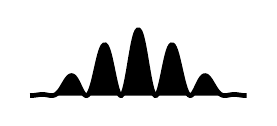
\begin{tikzpicture}[xscale=0.055,yscale=0.167]
	\draw [fill=black,line width=1.7pt,domain=-25:25,samples=200] plot (\x,{5*cos(deg(\x*3.14159/8))*cos(deg(\x*3.14159/8))*cos(deg(\x*3.14159/50))*cos(deg(\x*3.14159/50))});
\end{tikzpicture}
\end{textblock*}

\vspace*{0.3em}\hspace*{21em}$x$ (\si{\meter})
\end{document}
